\documentclass[runningheads,a5paper]{llncs}
\usepackage{graphicx}
\usepackage{tabularx}
\usepackage[latin1]{inputenc}
\usepackage{url}
\usepackage[normalem]{ulem}
\usepackage[ruled,vlined]{algorithm2e}
%\usepackage{float}

\urldef{\mailsa}\path|{jcgarcia,aespinosa}@caos.uab.cat| 
\urldef{\mailsb}\path|{juancarlos.moure,porfidio.hernandez}@uab.es|


\begin{document}

\mainmatter

\title{Search for Maximal Unique Matches in Multi-core architectures}
\author{Julio Cesar Garcia Vizcaino \and Antonio Espinosa \and Juan Carlos Moure \and Porfidio Hernandez }
 
 \authorrunning{Julio Cesar Garcia Vizcaino et al.}
 \institute{\footnotesize{Universitat Aut\'onoma de Barcelona (UAB), Barcelona, Spain}}

\maketitle
\begin{center}
  \mailsa

  \mailsb
\end{center}

\begin{abstract}
  Maximal Unique Matches (MUMs) are common substrings that match a Reference and a Query genome. They are exact, unique and maximal. The search for MUMs in large genomes is a heavy and repetitive task, so there is a fair chance of parallelize and execute this search in multi-core architectures. This research evaluates a parallelization of the search for MUMs in genomic sequences within multi-core architectures. The Reference genome is indexed by using a Suffix Tree or Enhanced Suffix Array in main memory and then a parallelized algorithm searches for MUMs between Reference genome and Query genome. Query genome is read by several threads in chunks of fixed size. This approach is based on MUMmer, a genome alignment tool, which is able to find Maximal Unique Matches (MUMs). Results show a reduction in search time and less usage of memory.

\keywords{Indexed Search, Bioinformatics, Maximal Unique Match, Multi-core architectures, Parallelization}
\end{abstract}

\section{Introduction} 
Modern sequencing and computational technologies and advances in bioinformatics has made whole genome sequencing possible. One resulting challenge is the fast alignment of whole genomes. Dynamic programming is too slow for aligning two large genomes, hundreds of Mbp. One very successful approach to perform a whole genome alignment is based on identifying ``maximal unique matches''. This heuristic is based on the assumption that one expects substrings occurring in two similar genomes. Maximal unique matches (MUMs) are almost surely part of a good alignment of the two sequences and so the whole genome alignment problem can be reduced to aligning the sequence in the gaps between the MUMs.
\begin{definition}
Assume we are given two sequences R,Q $\in \Sigma^*$, and a number L > 0. The maximal unique matches problem (MUM-problem) is to find all sequences u $\in \Sigma^*$ with: $|u|\geq L$, u occurs exactly once in R and once in Q, and for any character a $\in \Sigma^*$ neither ua nor au occurs both in R and Q.
\end{definition}
The problem of searching maximal unique matches for a minimum length between a Reference genome and a Query genome has been identified in several applications, one of them is MUMmer \cite{Delcher2003}. MUMmer's algorithm can perform searches for Maximal Unique Matches (MUMs), although with a high use of main memory to store the Reference genome and a null use of multi-core architectures.

We designed and tested a data-level parallelism to use in multi-core architectures with two different data structures: Suffix Tree and Enhanced Suffix Array.

The rest of this paper is organized as follows. Section 2 discusses the related work. Section 3 defines some definitions used in this paper. Section 4 shows our implementation of parallelization of search for MUMs. Section 5 discusses the results of our parallelization. Section 6 concludes the paper.
\section{Related work}
Search for Maximal Unique Matches to do Whole Genome Alignment was proposed in \cite{Delcher1999}. There have been some previous work in the parallelization of search of matches in genomic data, like \cite{OguzhanKulekci2011,Mongelli,Kouzinopoulos2005}, however these works are focused in fixed patterns and read alignment. On the other hand, there have been achievements in parallelization of Whole Genome Alignment like \cite{Meng2005}. The parallelization of searching for MUMs with a full-text index data structure is a research field not covered very deep, there is only one approach in \cite{Encarnac2011} but without access to source code to check their implementation and it is more focused with GPU and CPU hybrid architectures and Suffix Array. There are other implementations in \cite{Vyverman2013,OguzhanKulekci2011,Khan2009,OhlebuschGK10} but they search for Maximal Exact Matches with threads and not Maximal Unique Matches . We propose the use of OpenMP to search for MUMs in multi-core architectures with two full-text index data structures: Suffix Tree and Enhanced Suffix Array.
\section{Preliminaries}
Let's assume the Reference genome $R[0,\ldots, n-1]$ of size $|R|=n$ over an alphabet $\Sigma={ \$, A, C, G, T}$ which has a sentinel character $R[n-1] = \$$ that occurs nowhere else in the Reference genome and is lexicographically less than all the characters that occur in the alphabet. The suffixes of the Reference genome are zero indexed by their position in the original Reference by a full-text index data structure like a Suffix Tree or an Enhanced Suffix Array. 
\begin{definition}
A suffix Tree, $ST$, for an n-character string $R$ is a rooted directed tree with exactly $n$ leaves numbered 0 to n. Each internal node, other than the root, has at least two children and each edge is labeled with a nonempty substring of $R$. No two edges out of a node can have edge-labels beginning with the same character. For any leaf $i$, the concatenation of the edge-labels on the path from the root to leaf $i$ exactly spells out the suffix of $R$ that starts at position $i$. That is, it spells out $R[i\ldots n]$. \cite{Gusfield1997}.
\end{definition}
\begin{definition}
  An enhanced suffix array consists of four arrays (suffix, longest common prefix (LCP), child and inverse suffix arrays) that have parts of the information saved in a suffix tree. \cite{Abouelhoda2004}.
\end{definition}
We also define a suffix link, which an important trick to achieve linear complexity to search for MUMs in both Suffix Tree and Enhanced Suffix Array.
\begin{definition}
A suffix link is a pointer from string $\overline{aw}$ to substring $\overline{w}$.
\end{definition}
For reasons of space we recommend the reader to check \cite{Abouelhoda2004} for full description of Enhanced Suffix Array.
%\begin{definition}
%Given an n-character string $R$, a Suffix Array, $SA$, for $R$ is an array of the integers in the range 0 to $n-1$, specifying the lexicographic order of the $n$ suffixes of string $R$. \cite{Gusfield1997}.
%\end{definition}
A search for a MUM between a Reference genome, $|R|=n$, and a Query genome, $|Q|=m$,  can be done in a Suffix Tree in $O(m)$ steps and in an Enhanced Suffix Array in $O(m)$ steps.
%However it is possible to improve the search for MUMs in a Suffix Array by using an inverse Suffix Array, a LCP-table and a child table. These improvements reduce a $O(m)$ steps \cite{Abouelhoda2004} the complexity to search for MUMs using a Suffix Array.
%\begin{definition}
%An Inverse Suffix Array, $ISA$, is a table of size $n$ such that $ISA[SA[q]]=q$ for any $0\geq q> n$. \cite{Abouelhoda2004}.
%\end{definition}
%\begin{definition}
%A LCP-table, $LCP$, is an array of integers from 0 to n-1. Where $LCP[0]=0$ and $LCP[i]$ is the length of the longest common prefix of $SA[i-i]$ and $SA[i]$ for $1\geq i>n$. \cite{Abouelhoda2004}.
%\end{definition}
%\begin{definition}
%A child table, CHILD, is a table of size $n$ indexed from 0 to n-1 and each entry contains three values: up, down, and nextlIndex. These values are defined as follows: 
%
%CHILD[i].up = $min\{q\in [0\ldots i-1]|LCP[q]>LCP[i]\;and\;\\
%\forall k\in[q+i\ldots i-1]:LCP[k]\geq LCP[q]\}$,\\
%CHILD[i].down = $max\{q\in[i+1\ldots n]|LCP[q]>LCP[i]\\
%and\;\forall k\in[i+1\ldots q-1]:LCP[k]\geq LCP[q]\}$,\\
%CHILD[i].nextlIndex = $min\{q\in[i+1\ldots n]|LCP[q]=LCP[i]\\
%and\;\forall k\in[i+1\ldots q-1]:LCP[k]>LCP[i]\}$.
%\end{definition}
%\begin{definition}
%An $l-$interval $[i\ldots j]$ is an lcp-interval of lcp-value $l$ if\\
%$LCP[i]<l$\\
%$LCP[k]\geq l$ for $i<k\leq j$\\
%$LCP[k]=l$ for at least one $k$ in $i<k\leq j$\\
%$LCP[j+1]<l$
%\end{definition}
%To simulate a traversal of a Suffix Tree on an Enhanced Suffix Array we require the child table. In order to perform the traversal we get an interval $l-$interval $[i..j]$ and a character $a\in \Sigma$ as input and returns the child interval $[l..r]$ of $[i..j]$ whose suffixes have the character $a$ at position $l$. Note that all the suffixes in $[l..r]$ share the same $l-$character prefix because $[l..r]$ is a subinterval of $[i..j]$. This process is performed in $O(|\Sigma|)$ time.
%\begin{figure}[h]
%  \centering
%  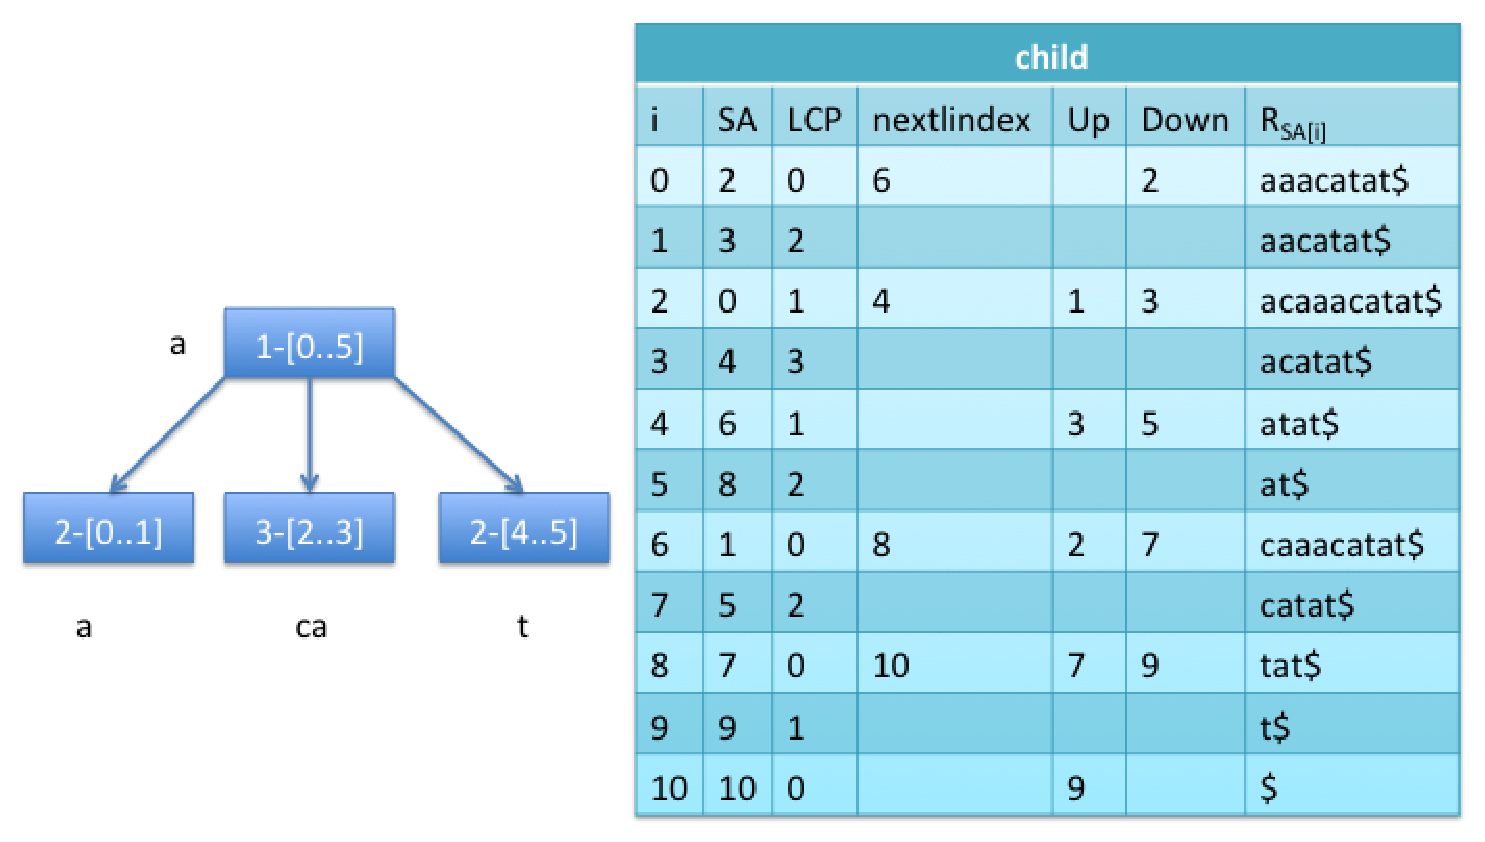
\includegraphics[scale=0.35]{child.eps}
%  \caption{Enhanced Suffix Array for string R=acaaacatat\$. Child interval 1-[0..5] where CHILD[6].up=2, CHILD[2].down=1, CHILD[2].nextlindex=4.}
%  \label{fig:esa}
% \end{figure}  
Once we have defined the resources used to index a Reference genome, we need to answer the question: Where are the MUMs of $R$ and $Q$ of some minimum length $L$? We show the algorithms used to answer this question using a Suffix Tree, see Algorithm \ref{algST}, and a Enhanced Suffix Array, see Algorithm \ref{algESA}.
\linesnumbered
\begin{algorithm}[h]
  \label{algST}
  \dontprintsemicolon
  \SetKwInOut{Input}{input}
  \SetKwInOut{Output}{output}
  \SetKwData{R}{R}
  \SetKwData{Q}{Q}
  \SetKwData{ST}{ST}
  \SetKwData{Len}{L}
  \SetKwData{Length}{length}
  \SetKwData{Leaf}{leaf}
  \SetKwData{MUMs}{MUMs}
  \SetKwData{MUMcands}{MUMcands}
  \SetKwFunction{buildST}{buildST}
  \SetKwFunction{TraverseSuffixTree}{TraverseSuffixTree}
  \SetKwFunction{isLeafNode}{isLeafNode}
  \SetKwFunction{saveMUMcand}{saveMUMcand}
  \SetKwFunction{cleanMUMcand}{cleanMUMcand}
  \Input{\R, \Q, \Len}
  \Output{List of \MUMs of \Length$\geq$ \Len, with start position in \R and \Q and \Length}
  \Begin{
  \ST$\leftarrow$ \buildST{\R}\;
  \ForEach{position $i\in Q$}{
  \Length$\leftarrow$ \TraverseSuffixTree{$\Q[i]$,\ST}\;
    \If{\isLeafNode{$\Q[i]$}}{
    \tcc{Leaf saves the position of a suffix in ST.}\;
        \If{$\R[\Leaf-1]\neq \Q[i-1]$ and $\Length\geq L$}{
            \MUMcands$\leftarrow$ \saveMUMcand{$\R_{\Leaf}$,$i$,\Length}\;
        }
    }
  }
  \tcc{Get unique MUMs from list of MUM-candidates.}\;
  \MUMs$\leftarrow$ \cleanMUMcand{\MUMcands}
  }
  \caption{Search for MUMs in a Suffix Tree.}
\end{algorithm}
\linesnumbered
\begin{algorithm}[h]
  \label{algESA}
  \dontprintsemicolon
  \SetKwInOut{Input}{input}
  \SetKwInOut{Output}{output}
  \SetKwData{R}{R}
  \SetKwData{Q}{Q}
  \SetKwData{Len}{L}
  \SetKwData{End}{end}
  \SetKwData{inter}{interval}
  \SetKwData{n}{n}
  \SetKwData{vi}{i}
  \SetKwData{sa}{SA}
  \SetKwData{esa}{ESA}
  \SetKwData{isa}{ISA}
  \SetKwData{qF}{queryFound}
  \SetKwData{MUMcands}{MUMcands}
  \SetKwFunction{tra}{traverseESA}
  \SetKwFunction{saveMUMcand}{saveMUMcand}
  \SetKwFunction{cleanMUMcand}{cleanMUMcand}
  \SetKwFunction{bESA}{buildESA}
  \SetKwFunction{sufl}{suffixlink}
  \SetKwFunction{lfmax}{leftMaximal}
  \SetKwData{Length}{length}
  \SetKwData{MUMs}{MUMs}
  \Input{\R, \Q, \Len}
  \Output{List of \MUMs of \Length$\geq$ \Len, with start position in \R and \Q and \Length}
  \Begin{
  \esa$\leftarrow$ \bESA\;
  \While{\Q[\vi] $<$ \End} {
%    \tcc{Traverse ESA top down until mismatch or full string is matched.}\;
    \tra{\Q, \Q[i], \inter, \Q[\vi].length()}\;
    \If{\inter.depth $\leq$ 1} { 
       \inter.depth = 0; \inter.start = 0; \inter.end = \n-1; \vi++; continue; }
    \If{\inter.size() == 1 and \inter.depth $\geq$ \Len} {
      \If{\lfmax{\Q, \Q[\vi], \sa[\inter.start]}} {
            \saveMUMcand{\sa[\inter.start],\vi,\inter.depth}\;
      }
    }
    \Repeat{\inter.depth $>$ 0 and \inter.size()} {
      \inter.depth = \inter.depth-1\;
      \inter.start = \isa[\sa[\inter.start] + 1]\;  
      \inter.end = \isa[\sa[\inter.end] + 1]; 
      \vi++;
      \If{\inter.depth == 0 or \sufl{inter} == false} { \inter.depth = 0; \inter.start = 0; \inter.end = \n-1; break; }
    } 
  }
  \MUMs$\leftarrow$ \cleanMUMcand{\MUMcands}
  }
  \caption{Search for MUMs in an Enhanced Suffix Array.}
\end{algorithm}
\section{Implementation}
The search for MUMs between a Reference and Query genome has an important feature which may help us to parallelize these algorithms: we can check more than one suffix of Query genome at the same time in Reference genome. Using a full-text index data structure to search for MUMs, we find MUM candidates while we stream the Query genome against the data structure. A MUM candidate is a MUM which is not unique in Query genome but only in Reference genome. To get a MUM we require to reach the end of Query genome to discard those MUM candidates which are not unique in both Reference and Query genome. Our approach, see Figure \ref{phases}, is divided in three phases: Creation of Suffix Tree or Enhanced Suffix Array; Splitting query genome data (chunks) according to the number of available cores using 1 thread per core and parallel execution of the search for MUMs for every chunk, then every thread has its own list of MUM candidates; and Get MUMs from list of MUM candidates of all threads. 
\begin{figure}
\centering 
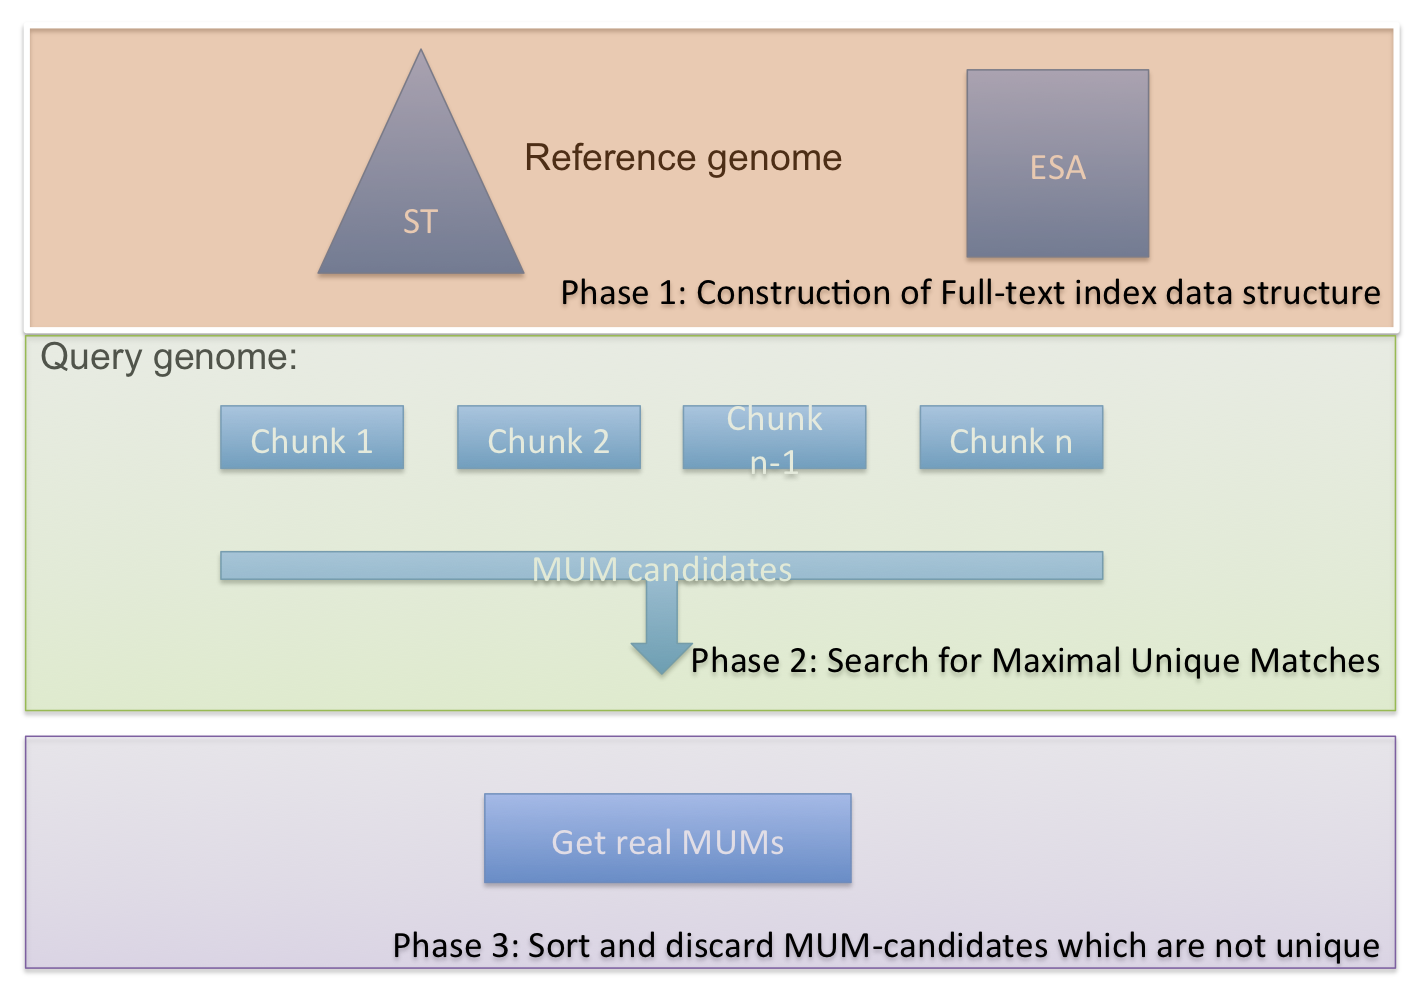
\includegraphics[scale=0.5]{phases.eps}
\caption{Approach to search for MUMs in multi-core architectures with Suffix Tree or Enhanced Suffix Array.}
  \label{phases}
\end{figure}
A data-level parallelism to search for MUMs requires to split the Query genome in chunks and stream each chunk against the full-text index data structure. This search is independent of each other chunk. The final stage to filter MUMs must be performed with a full Query genome and with chunks of Query genome is more obvious too. This approach is suitable to be performed in multi-core architectures because chunks can be assigned to each core and search for MUMs in the full-text index data structure which is stored in main memory. So that a very good choice of parallelization involves a data partition technique.

Memory usage is improved, within this approach, with multiple reads to the full-text index data structure, instead of one read at a time with a serial execution.We take advantage of multi-core architectures with our approach. Since a SPMD paradigm is used to solve the MUM-problem, we must tackle the common issues which arise when using multi-core architectures: cache issues, memory bandwidth and multithreading.

The division of Query genome uses the paradigm of data-level parallelism which consists of a generation of chunks of a Query genome with a fixed size. The chunk size was computed with Query genome length divided by number of available threads. Chunk size is a performance factor because we need to have a balanced workload among threads.

Phase 1 is the construction of the data structure: Suffix Tree or Enhanced Suffix Array; this phase is executed in a serial way. Phase 2 requires the parallel execution of the Algorithm (\ref{algST} or \ref{algESA}) to search for MUMs, the first step in Phase 2 is the split of Query genome in as many chunks as available threads. The split defines the start and end position in Query genome which is held in main memory and shared by all threads. The chunk size is fixed according to the number of threads. The parallel search for MUMs gets a list of MUM-candidates which are ordered in each thread by its position in Query genome. Phase 3 is performed after all threads have finished its execution and it merges the lists of MUM-candidates and it is ordered by position in Query genome (this step is needed because the merge process may have unordered lists); this unique list is checked to discard those MUM-candidates which are not unique in the Query genome. This check is performed in a serial way.

We evaluated two different full-text index data structures: a Suffix Tree and an Enhanced Suffix Array. We applied our approach, Figure \ref{phases}, by using OpenMP in the phase 2: search for MUMs with a static OpenMP schedule.
\section{Results}
To verify that our approach, can have a better performance to search for MUMs of a Reference and Query genome, in Table \ref{genomes}, we verify that output of MUMmer and our approach have the same MUMs. Tests were carried out in the following node: 2 Processor Intel(R) Xeon(R) E5645 @ 2.4GHz of 6 cores each one, 32KB L1 cache, 256KB L2 and 12MB L3 shared cache per socket. RAM: 96 GB. GCC 4.7.0 with OpenMP support + Linux. 
\begin{table} 
\centering
\caption{List of Genomes used in experiments.}
\label{genomes}
\begin{tabular}{|c|l|l|l|} \hline
  & 1 & 2 & 3 \\ \hline
  Reference & 4.64 [Mbp] & 169 [Mbp] & 1031 [Mbp] \\ \hline
  Query & 5.5 [Mbp] & 167 [Mbp] & 1357 [Mbp] \\ 
  \hline
\end{tabular}
\end{table}
The main goal of these tests was to check the performance to search for MUMs in multi-core architectures by using OpenMP (threads). This performance involves the usage of Memory and CPU (execution time to search for MUMs).\\
%One key aspect of the several tests executed was to assure the execution of every thread in a single core, that is no other thread is competing for the same cache. With affinity we ensure the scalability of our proposal, without affinity even a number of threads below the number of cores might be in the same core. \\
Times were collected during the execution of the experiments: construction time of data structure and execution time to search for MUMs with the function omp\_get\_wtime of OpenMP.\\
\subsection{Construction of Full-text index data structure}
This paper compares the performance of two data structures to search for MUMs in multi-core architectures, two features for these structures are: construction time and memory footprint. Full-text indexes allow fast access to substrings of any length, but they have a great memory and construction cost. This cost is affected by the type and implementation of the full-text index data structure used. 
We measure the construction time for the set of genomes in Table\ref{genomes}. Figure \ref{fig:construction} shows that an ESA has a lower construction time for all the Reference genomes used. Since a full-text index data structure has to be build every time a search for MUMs is performed, a reduction in the construction phase in Figure \ref{phases} would allow us to improve the overall execution time. A future improvement would be to build the full-text index data structure in parallel or load from a file.
 \begin{figure}[!htbp]
  \centering
  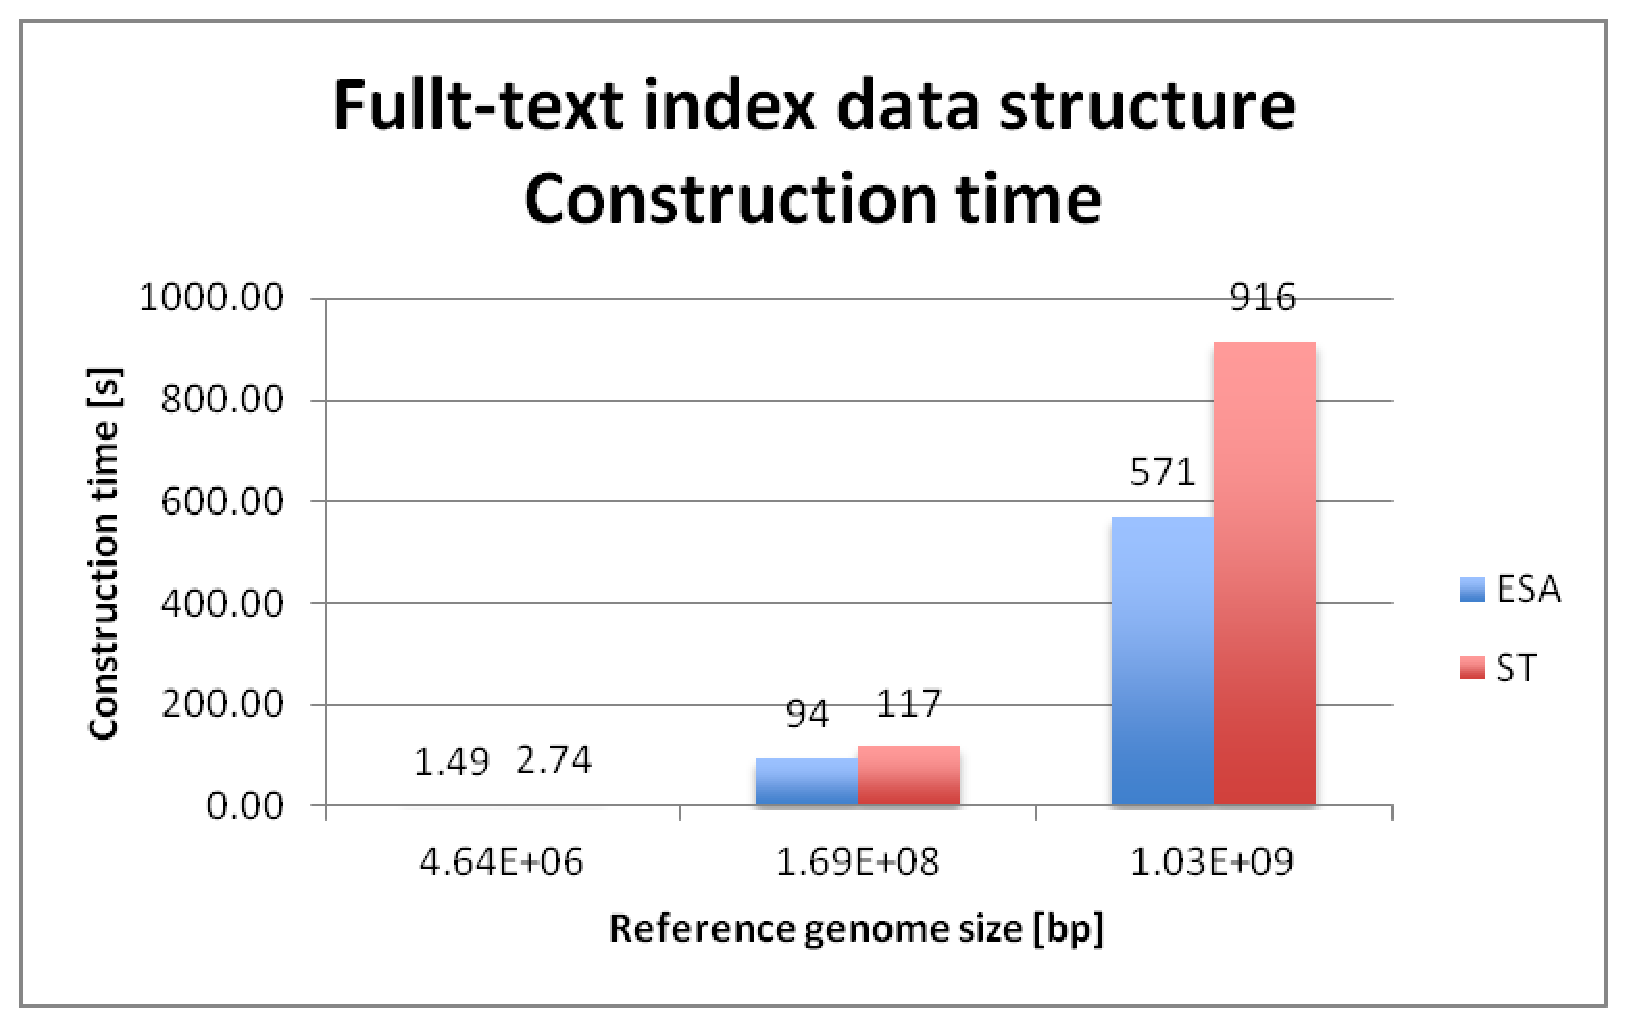
\includegraphics[scale=0.3]{construction.eps}
  \caption{Construction of Suffix Tree and Enhanced Suffix Array for several genomes sizes. Our approach stores the whole Reference genome indexed by a Suffix Tree (ST) or an Enhanced Suffix Array (ESA) in main memory.}
  \label{fig:construction}
 \end{figure}  
%\vspace{1cm}
 \subsection{Search for MUMs in multi-core architectures}
We focus in the experiment to search for MUMs of minimum length 20[bp]. Our goal is to get the best performance of a multi-core architecture while searching for MUMs with a Suffix Tree and Enhanced Suffix Array.
\subsubsection{EcoliK12 vs. EcoliO157H7}
The set 1 in Table \ref{genomes} was used to search for MUMs in a ST and ESA. In Figure \ref{fig:ecoli-mum}, we show that ESA has a better search time, see Figure \ref{fig:ecoli-mum}.
 \begin{figure}[!h]
  \centering
  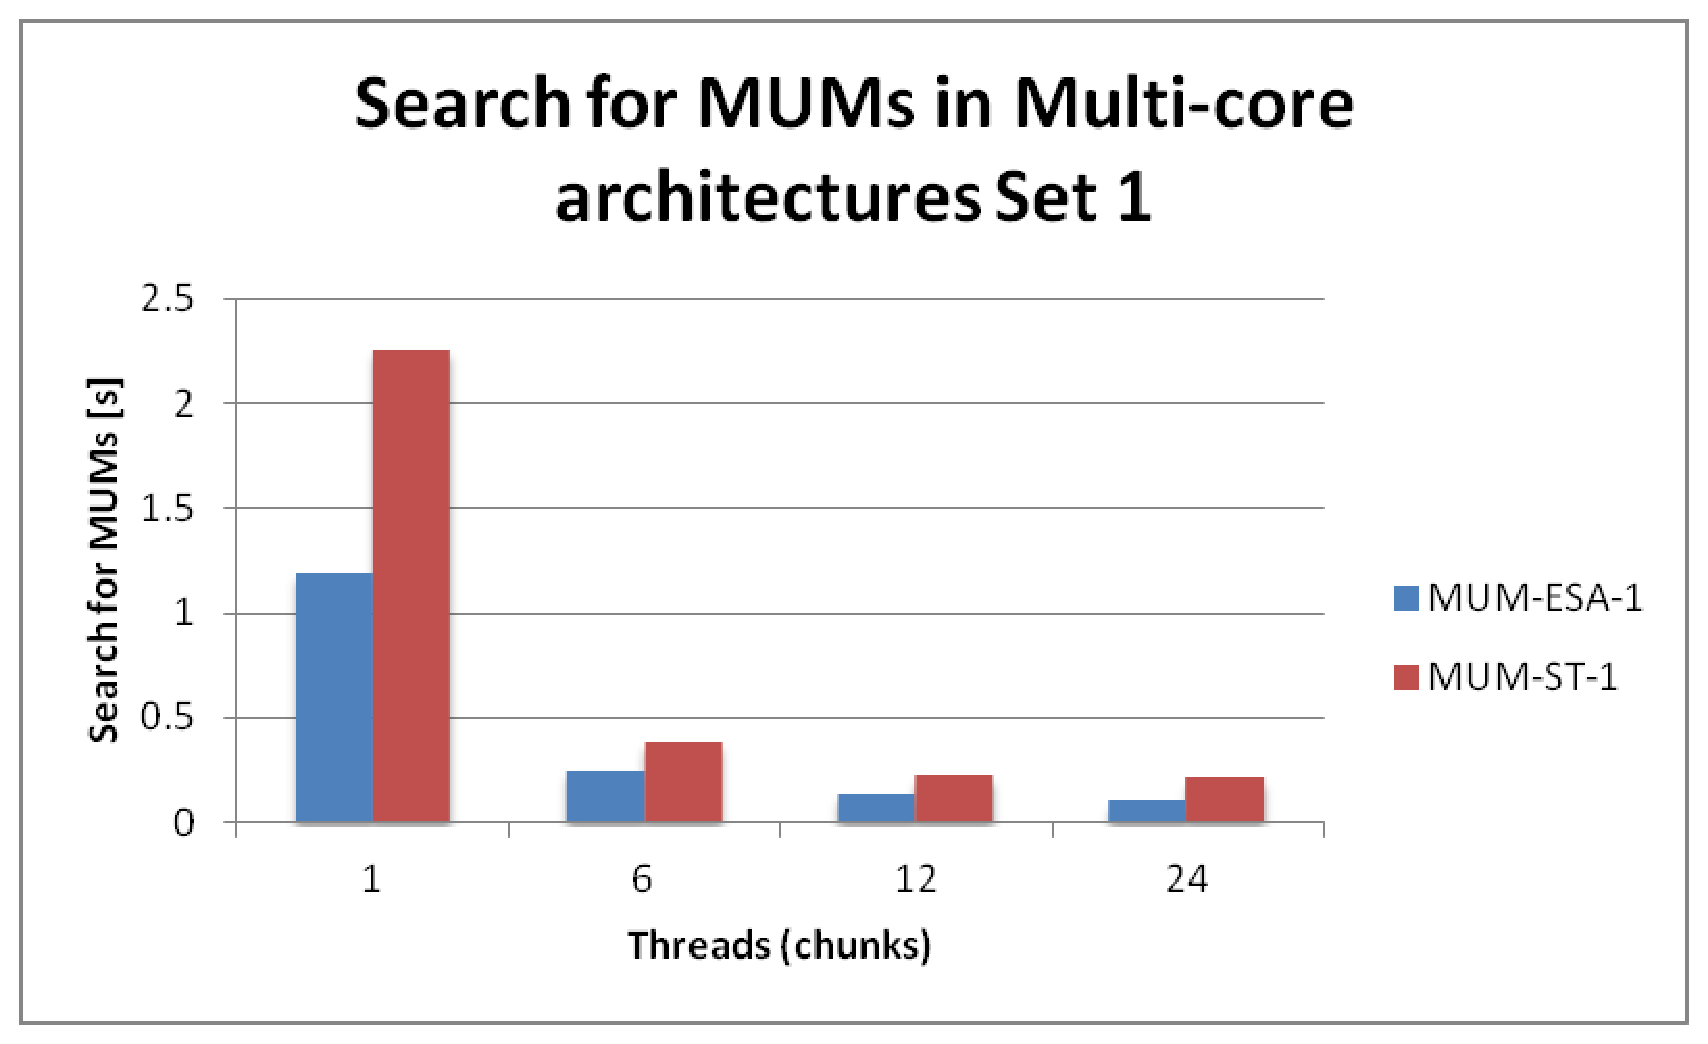
\includegraphics[scale=0.3]{ecoli-MUM.eps}
  \caption{Search for MUMs time for Ecolik12 and EcoliO157H7 in multi-core architectures with ST and ESA.}
  \label{fig:ecoli-mum}
\end{figure}  
However, the space consumption shows that ESA has a better memory footprint, a reduction of 44\% of memory space compare to Suffix Tree (159 MB).
%\begin{figure}[h]
%  \centering
%  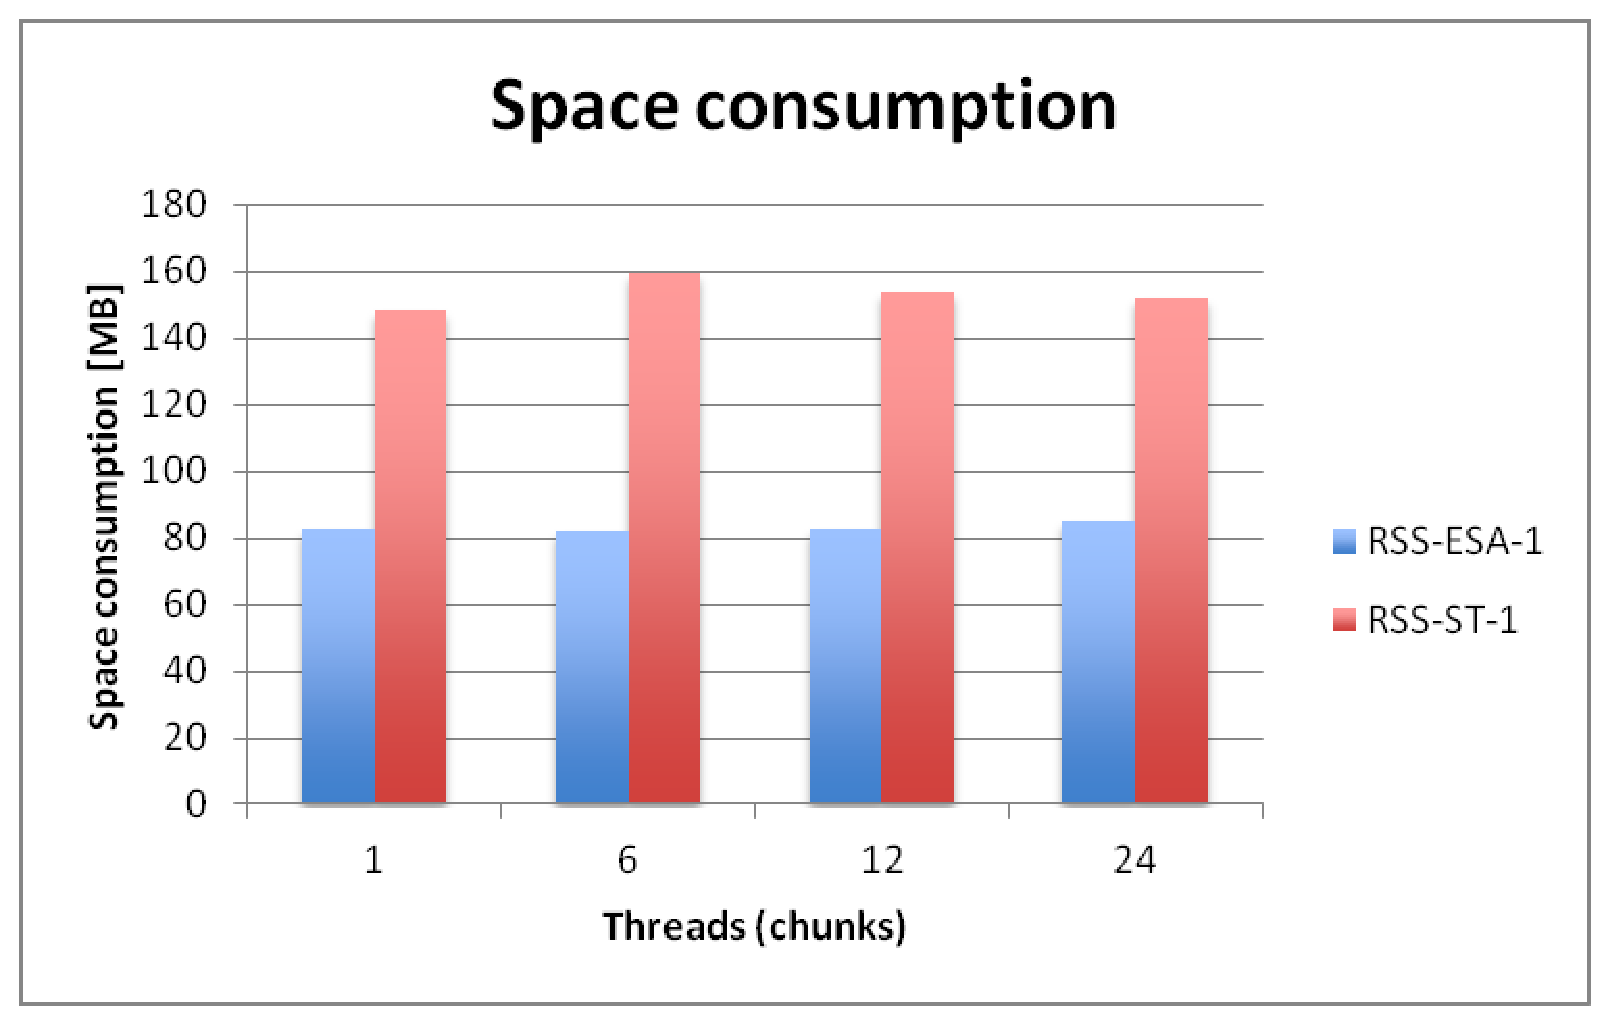
\includegraphics[scale=0.3]{ecoli-RAM.eps}
%  \caption{RAM consumption to search for MUMs for Ecolik12 and EcoliO157H7 in multi-core architectures with ST and ESA.}
%  \label{fig:ecoli-ram}
%\end{figure}  
This first experiment shows that it is possible to search for MUMs with two different full-text index data structures with thea reduction in search time but with a lower memory consumption for ESA.
\subsubsection{D.melanogaster vs. D.pseudoobscura}
The set 2 in Table \ref{genomes} increases the genome size and we show in Figure \ref{fig:fly-mum} that ESA has a smaller search time.
 \begin{figure}[!h]
  \centering
  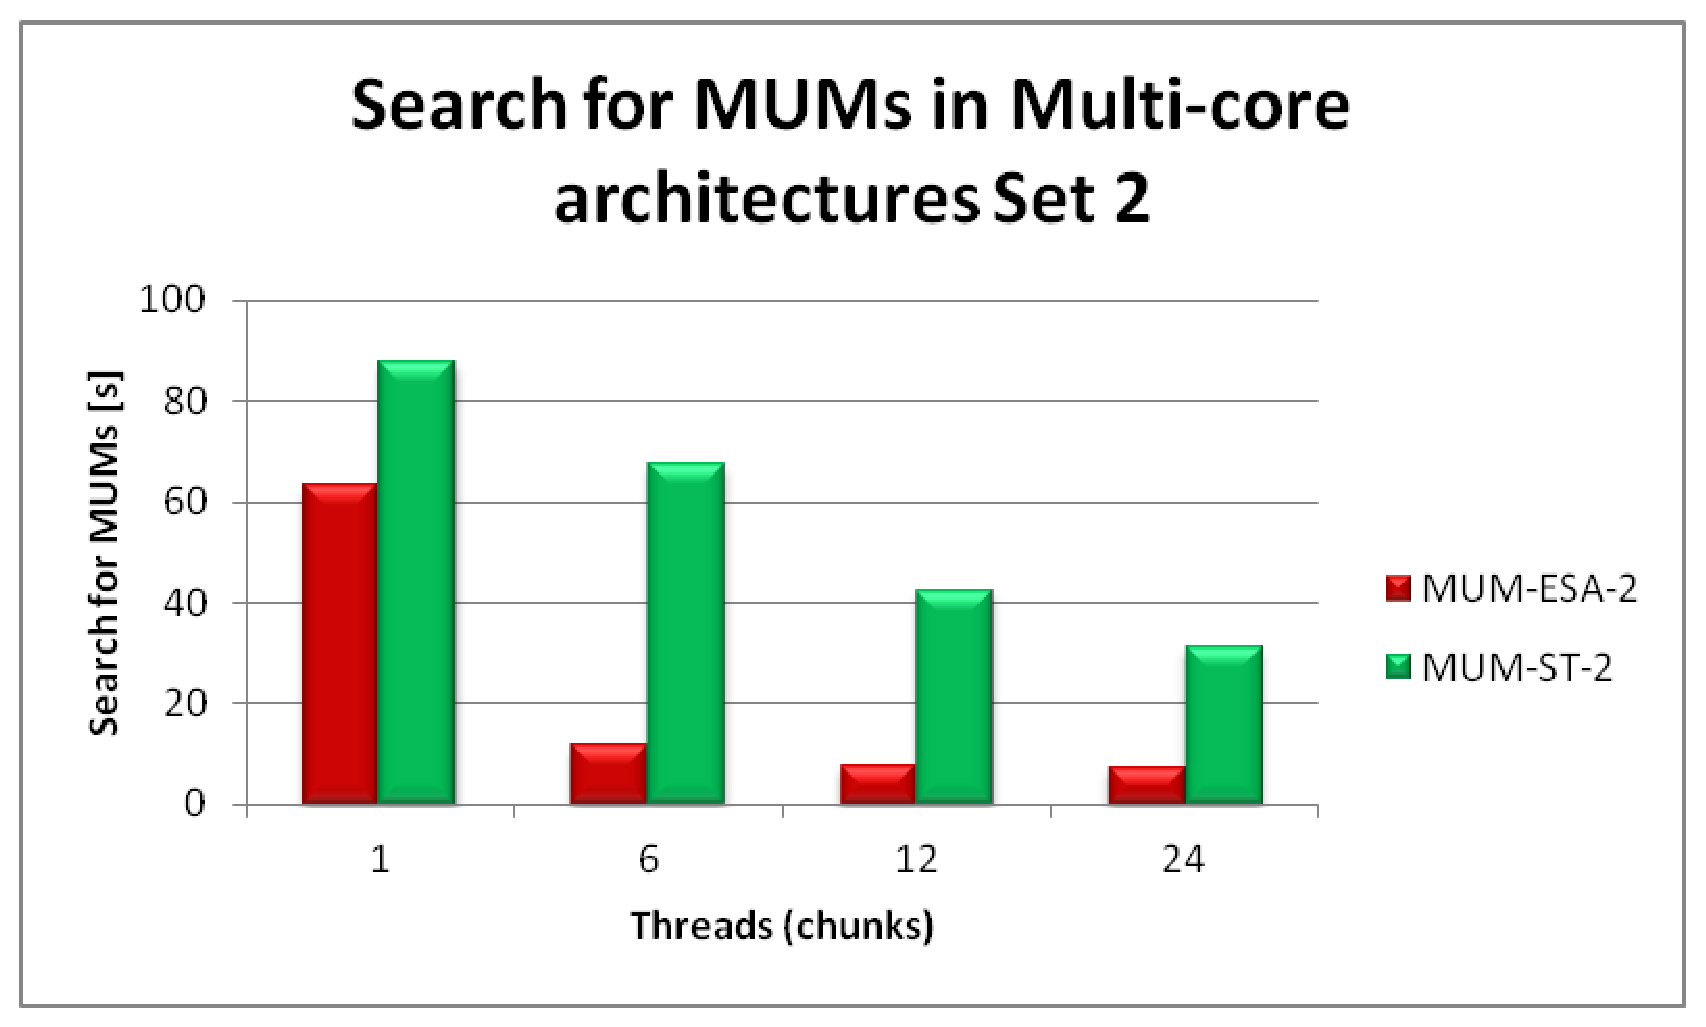
\includegraphics[scale=0.3]{fly-MUM.eps}
  \caption{Search for MUMs time for D.melanogaster and D.pseudoobscura in multi-core architectures with ST and ESA.}
  \label{fig:fly-mum}
\end{figure}  
However, there is a problem with scalability between 12 and 24 threads. Our approach does not scale good with ESA. Although ST has a better speedup, we require to reduce the search time.
On the other hand, the space consumption is almost constant in both data structures. However, again ESA has a better usage of memory. The reduction in memory footprint for ESA is near to the half of the ST.%, see Figure \ref{fig:fly-ram}.
%\begin{figure}[h]
%  \centering
%  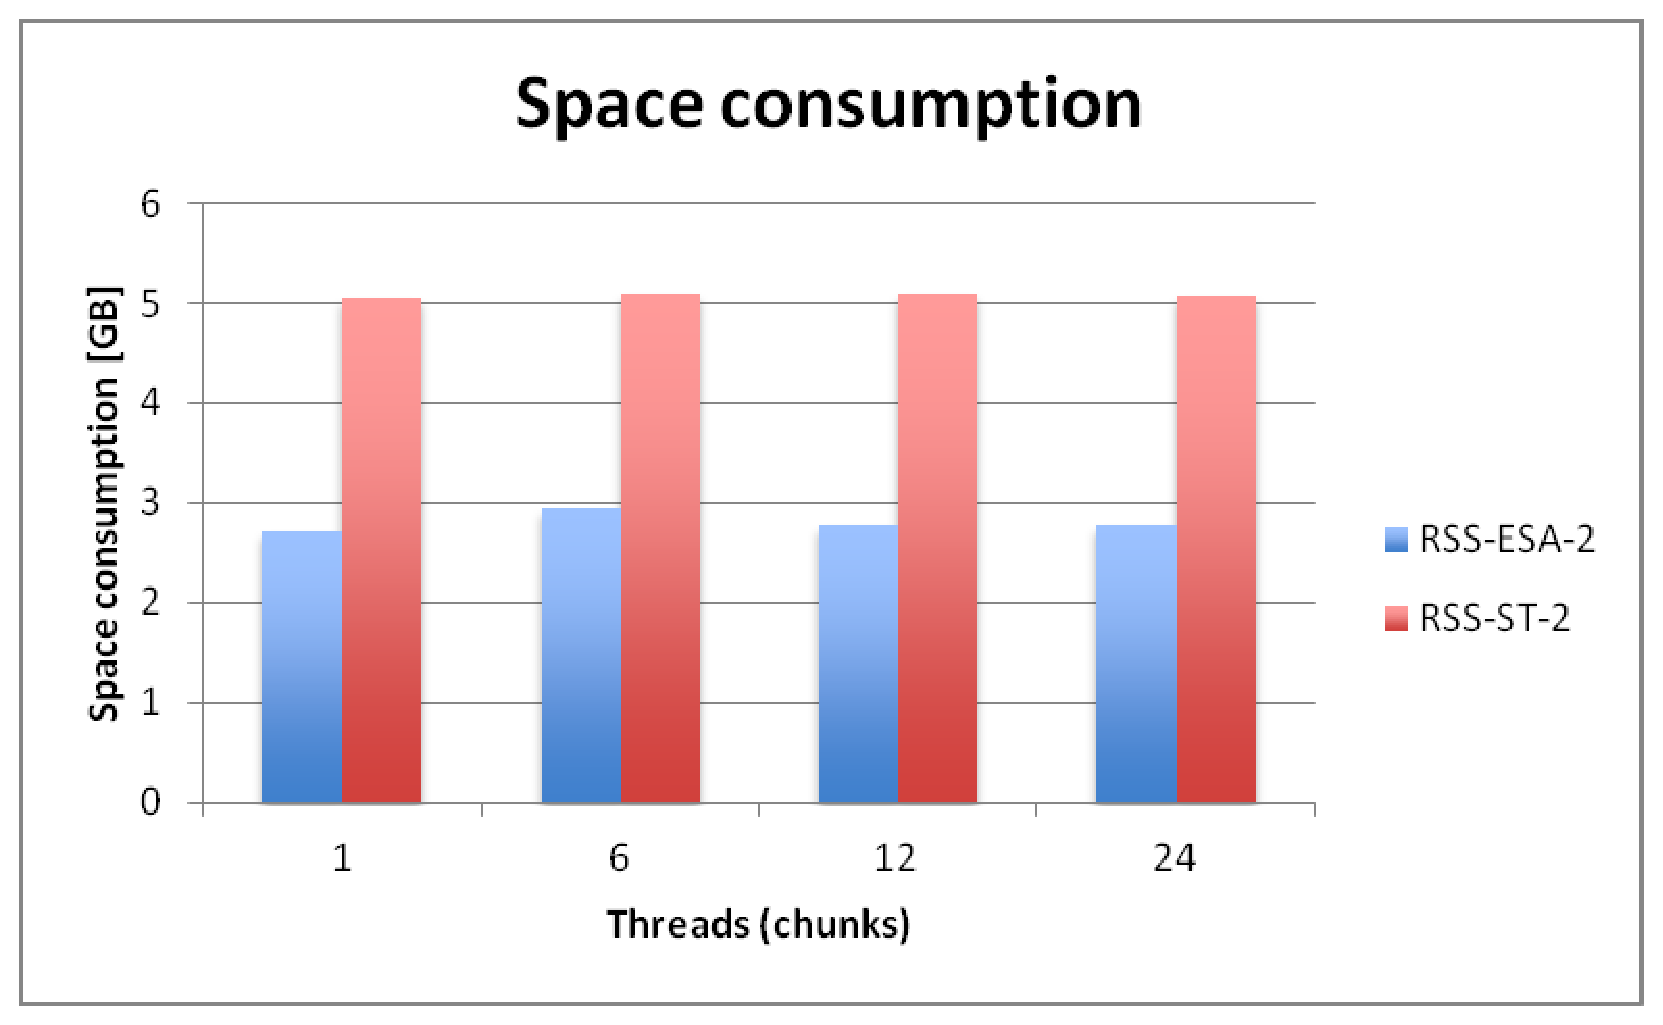
\includegraphics[scale=0.3]{fly-RAM.eps}
%  \caption{RAM consumption to search for MUMs for D.melanogaster and D.pseudoobscura in multi-core architectures with ST and ESA.}
%  \label{fig:fly-ram}
%\end{figure}  
\subsubsection{Chicken vs. Zebrafish}
The set 3 in Table \ref{genomes} have genomes of more than 1 [Gbp] and we show in Figure \ref{fig:chicken-mum} that an execution with one thread has a better performance in search time in ESA over ST. 
 \begin{figure}[!h]
  \centering
  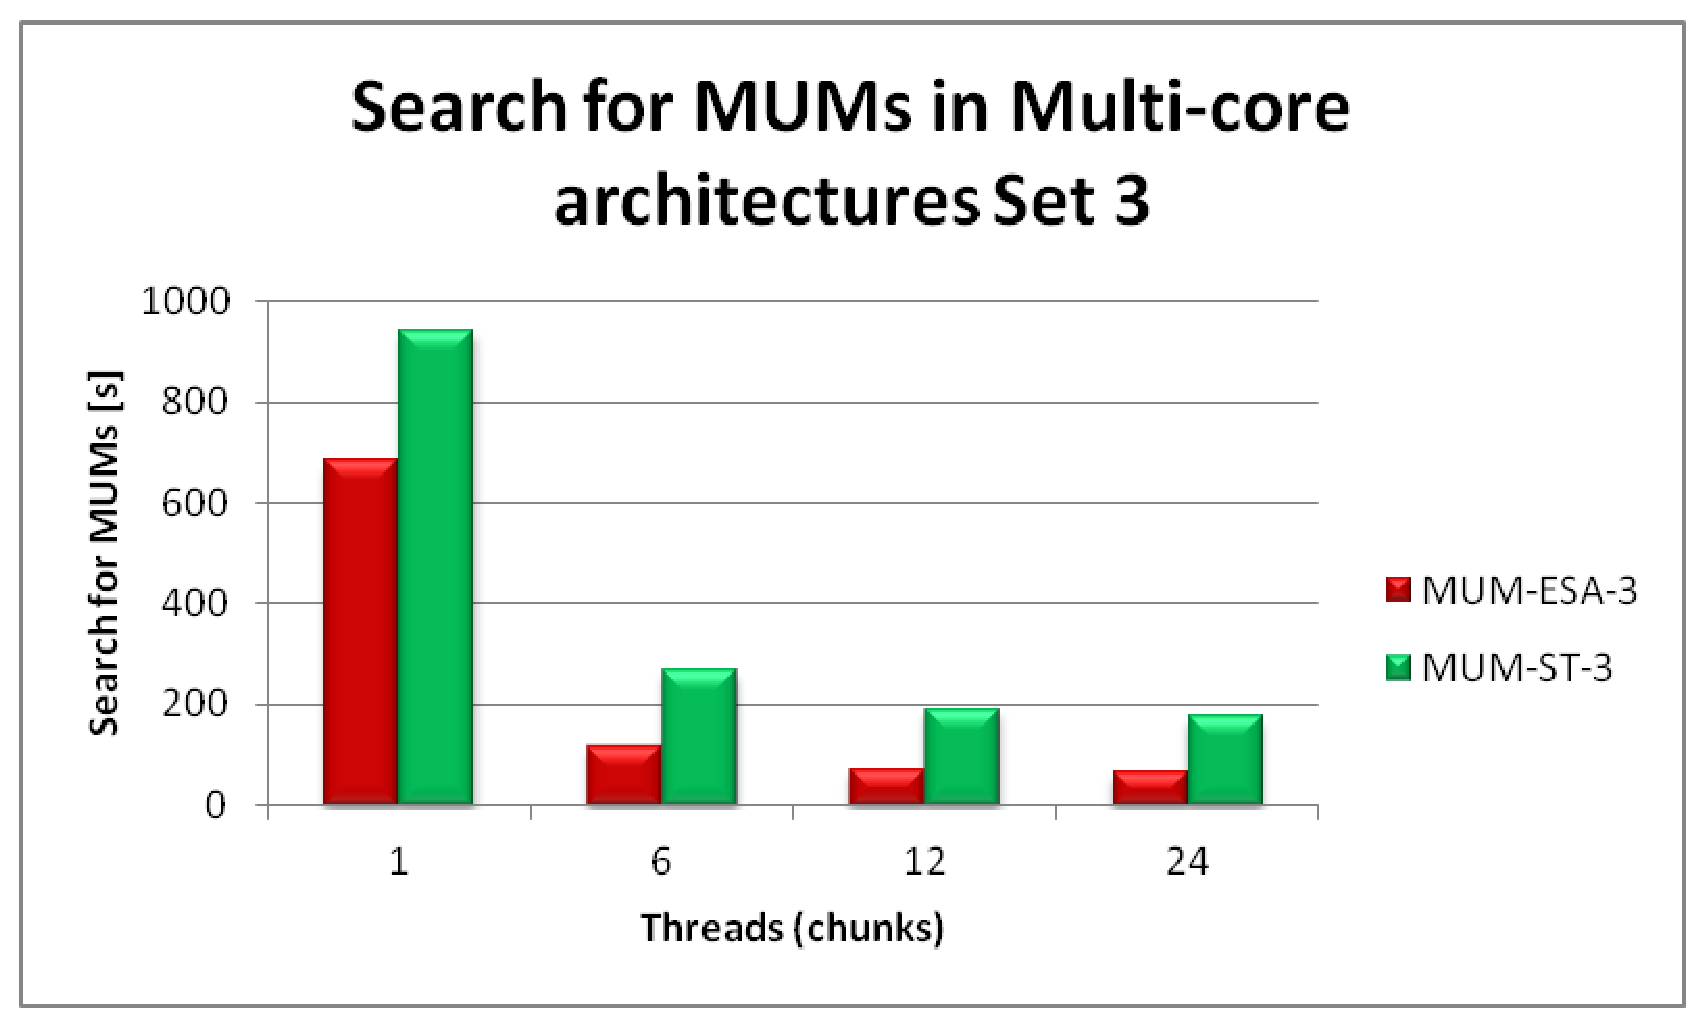
\includegraphics[scale=0.3]{chicken-MUM.eps}
  \caption{Search for MUMs time for Chicken and Zebrafish in multi-core architectures with ST and ESA.}
  \label{fig:chicken-mum}
\end{figure}  
In order to understand which full-text index data structure (ST, ESA) use to search for MUMs we check the memory footprint in Figure \ref{fig:chicken-ram}. The ESA has a better use of memory with the same search time.
 \begin{figure}[!h]
  \centering
  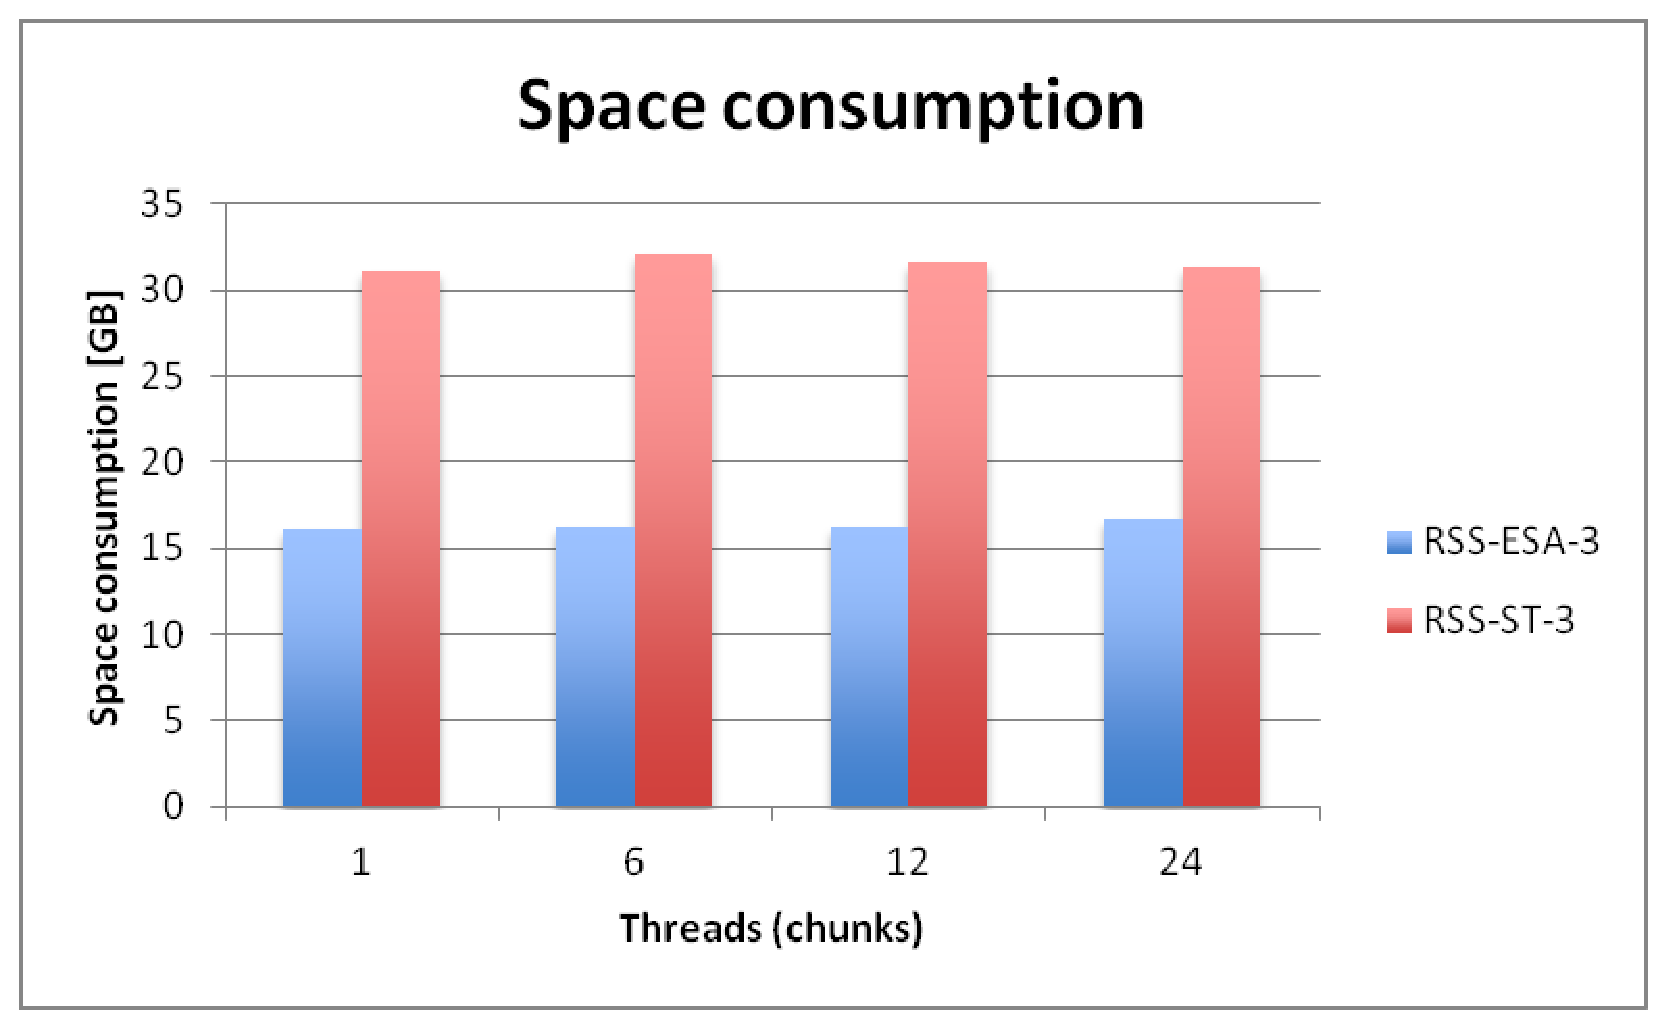
\includegraphics[scale=0.3]{chicken-RAM.eps}
  \caption{RAM consumption to search for MUMs for Chicken and Zebrafish in multi-core architectures with ST and ESA.}
  \label{fig:chicken-ram}
\end{figure}  
\section{Conclusions}
This paper presents an evaluation of performance to search for MUMs between Reference genome and Query genome in multi-core architectures with OpenMP in a Suffix Tree and an Enhanced Suffix Array. The search for MUMs is performed in a Suffix Tree or an Enhanced Suffix Array and the list of MUMs can help in the process of Whole Genome Alignment. The results show that MUM-problem can be solved with a ST or ESA and with the use of a multi-core architecture we reduce the execution time. There is a reduction in memory usage with an Enhanced Suffix Array over a Suffix Tree. We have evaluated a different data structure which provides the same functionality of a Suffix Tree to search for MUMs, with less use of memory in multi-core architectures.

Improvements involve a better use of CPU when we have more than one thread per core. From the results obtained we conclude that an Enhanced Suffix Array is suitable to solve the MUM-problem. To improve the performance in CPU usage of our approach, the following proposals may be used: Prefetching: this may work because we know in advance what intervals to look for in ESA and Query genome; Data cache management: we may need to store the interval of ESA in some cache-level of processor. Since we need to get the interval of search by checking the first character of the suffix within the interval, we may use some SSE instructions to check more than one suffix at the same time.
\section{Acknowledgments}
This work was supported by grant from "Ejecuci\'on eficiente de aplicaciones multidisciplinares: nuevos desaf\'ios en la era multi/many core", with reference TIN2011-28689-C02-01.
\bibliographystyle{abbrv}
\bibliography{mum-mc}  
\end{document}
